\documentclass[../main.tex]{subfiles}

\graphicspath{{../images/}}

\begin{document}

\section*{481 Lecture 1/16/24}
\barh \vspace{10px}
\section{Chapter 1: Probablities and Interference (Mackay Ch 2-3)}
\barh

\paragraph{An ensemble: $x$ random variable}

\begin{align*}
    A_x &= (a_1, a_2, \dots, a_n) \\
    P_x &= (p_1, p_2, \dots, p_n) \\
    &p(x = a_i) = p_i 
\end{align*}
$x$ takes value $a_i$ with probability $p_i$
\begin{align*}
    p \geq 0, \quad \sum_{a_i \in A_x} p(x = a_i) = 1
\end{align*}

Short hand for $p(x = a_i)$ is $p(a_i), \quad p(x)$

Joint ensemble: $X, Y$ ensembles
\begin{align*}
    XY &= \text{ordered pairs} (x, y) \quad x \in A_X, y \in A_Y \\
    P(x,y) &= \text{joint probability of x and y} 
\end{align*}

Marginal probability: $P(x,y) \rightarrow P(x), P(y)$
\begin{align*}
    P(x) &= \sum_{y \in A_y} P(x,y) \\
    P_x(x = a_i) &= \sum_{b \epsilon A_y} P_{XY}(x = a_i, y = b)
\end{align*}

Conditional probability: 
\begin{align*}
    P(x = a_i | y = b_j) = \frac{P(x = a_i, y = b_j)}{P(y = b_j)} 
\end{align*}
``Probability of $x = a_i$ given that $y = b_j$ (is true)''

\paragraph{Example 1}
$XY = 2$ successive letters in english alphabet.
$P_x$ and $P_y$ are identical `frequency of a letter in english'
\begin{align*}
    A_{xy} &= \{aa, ab, ac, \dots, zz\}
\end{align*} 

\begin{align*}
    P(y | x = `q') 
\end{align*}
Peak at $y = `u'$
\begin{align*}
    \neq P_Y(y)
\end{align*}
because $x$ and $y$ are not independent

$X,Y$ ``independent'' if (and only if) $P(x,y) = P(x)P(y)$

Userful relations: $P(x, y) = P(x | y) P(y) = P(y | x) P(x)$

For any assumption H
\begin{align*}
    \forall H : \qquad P(x,y | H) = p(x, y | H) p(y | H)
\end{align*}

`Sum rule':
\begin{align*}
    P(x | H) = \sum_{y \in A_y} P(x,y | H) = \sum_{y \in A_y} P(x | y, H) P(y | H)
\end{align*}

\newpage
\section{Lecture 1/18}
\hrule \vspace{10px}

\paragraph{Last time:} Main point $P(y|x) \neq P(y)$

Useful relations: Conditional probability
\begin{align*}
    P(x|y) = \frac{P(x,y)}{P(y)}
\end{align*}
where the joint relation is 
\begin{align*}
    P(x,y) = P(x|y) P(y) = P(y|x) P(x)
\end{align*}
this can be rewritten into \emph{Baye's theorem}
\begin{align*}
    P(y|x) = \frac{P(x|y) P(y)}{P(x)}
\end{align*}

\paragraph{Example 2:} Apply Baye's theorem
Alex is test for a nast disease.
\begin{itemize}
    \item Disease status: $a$ (sick or healthy)
    \item Test outcome: $b$ (positive or negative)
\end{itemize}
``Test is 95\% reliable'' or
\begin{align*}
    P(+|\textrm{sick}) = 0.95, \quad P(-|\textrm{healthy}) = 0.95
\end{align*}
Disease is nasty but rare $P(\textrm{sick}) = 0.01$; $P(\textrm{Healthy}) = 0.99$\\
Test is positive, what is the probability that Alex is sick? $P(\textrm{sick}|+)=?$
\subparagraph*{Solution} Use Baye's theorem:
\begin{align*}
    P(\textrm{sick}|+) = \frac{P(+|\textrm{sick}) P(\textrm{sick})}{P(+)}  
\end{align*}
where $P(+)$ is the probability of a positive test result. This can be found using the sum rule
\begin{align*}
    P(+) = P(+|\textrm{sick}) P(\textrm{sick}) + P(+|\textrm{healthy}) P(\textrm{healthy})
\end{align*}
Thus
\begin{align*}
    P(\textrm{sick}|+) = \frac{0.95*0.01}{0.95*0.01 + 0.05*0.99} = 0.161
\end{align*}
% 3x3 table
It is useful to write the probabilities in a table
\begin{center}
    \begin{tabular}{c|c|c|c}
        & $b = +$ & $b = -$ & $P(b)$ \\
        \hline
        $a = \textrm{sick}$ & $0.95*0.01$ & $0.05*0.01$ & $0.01$ \\
        $a = \textrm{healthy}$ & $0.05*0.99$ & $0.95*0.99$ & $0.99$ \\
        \hline
        $P(a)$ & $0.161$ & $0.839$ & $1$
    \end{tabular}
\end{center}
where columns represent the 95:5 reliable test.
\paragraph{Exclam!}
\begin{align*}
    P(S|+) \neq P(+|S)
\end{align*}

\paragraph{A brief philosphical interlude\dots}
The `Bayesian viewpoint':

Probability as degree of beliefs in propositions given assumptions \& evidence, or 
Probability as `freq of outcomes in repeat random experiments'

\subsection*{Forward and inverse problems}

So far we have talked about Cond Prob, Baye's thrm, and and example.

\paragraph{Generative Model:} Parameters $\Theta \rightarrow P(D|\Theta) \rightarrow (P)$ outcomes
(data) AKA `forward problem'

`a model' predicts an outcome given parameters. The model is a probablity distribution due to all 
the uncertainties and errors we have in the real world. 

\paragraph{The Inverse Problem} $P(\Theta|D)$

The inverse problem is the opposite of the forward problem (obviously). Also related to the issues
regarding `inference' and using Baye's theorem.

\paragraph{Example 3:} A forward problem

An urn contains $K$ balls, $B$ balls are black, and $K-B$ balls are white. A ball is drawn at $N$
times with replacement.

\begin{itemize}
    \item $n_B = $ \# of times a black ball is drawn 
    \item $P(n_B)$, average $n_B$?, STD?
\end{itemize}
With
\begin{align*}
    f_B = \frac{B}{K}
\end{align*}
The probability is given by the binomial distribution
\begin{align*}
    P(n_B|N,f_B) = \binom{N}{n_B} f_B^{n_B} (1-f_B)^{N-n_B}
\end{align*}
The mean is $N*f_B$ and the STD is $\sqrt{N*f_B*(1-f_B)}$

\paragraph{Example 4:} An inverse problem

We have 11 urns, each with 10 balls. $u$ is the number of black balls in each urn and the
urns have $u = 0, 1, \dots, 10$ black balls. Alex selects an urn at random and draws $N$ balls 
at random with replacement.
Bob wates Alex, but does not know which urn $u$ was selected. For Bob, what is 
$P(u|N,n_B)$?

\emph{We have the data, but we are trying to infer the parameter $u$}

\subparagraph*{Solution} Use Baye's theorem

\begin{align*}
    P(u|N,n_B) = \frac{P(n_B|u) P(u)}{P(n_B)}
\end{align*}
where $P(n_B|u)$ is the `forward' part from Ex 2, $P(u) = 1/11$, and $P(n_B)$ is the `normalization'
that makes it a valid prob. distribution:
\begin{align*}
    P(n_B) = \sum_{u'} P(n_B|u') P(u')
\end{align*}
Therefore
\begin{align*}
    P(u|N,n_B) \propto \binom{N}{n_B} \qt(\frac{u}{10})^{n_B} \qt(1-\frac{u}{10})^{N-n_B}
\end{align*}
e.g. $n_B = 3, N = 10$

\emph{insert figure 1.2}

The (0,0) point is impossible because we picked 3 black balls, and the urn $u=0$ has no black balls.
The same is true for the (10,10) point. The most likely point is $u=3$\dots

\subparagraph*{Exclam!}

This is known as `Posterior Probabilty'
\begin{itemize}
    \item $\Theta$ is the parameter
    \item $D$ is the data
    \item $P(\Theta)$ is the prior
    \item $P(D|\Theta)$ is the likelihood: a function of $D$ prob of data given param \\
        (sums to 1 over all options for $D$). As a function of $\Theta \rightarrow$
        likelihood of $\Theta$ 
    \item $P(\Theta|D)$ is the posterior
    \item $P(D)$ is the normalization
    \item [!] \textbf{Probability of \emph{data}}
    \item [!] \textbf{Likelihood of \emph{parameters}}
\end{itemize}


\paragraph{Role of Prior:}
\begin{itemize}
    \item[!] You can't do inference without making assumptions
\end{itemize}

\newpage
\section*{Lecture 1/23/24}
\barh \vspace{10px}

\paragraph{Last time: }
\begin{itemize}
    \item Forward $p(data | param)$
    \item Inverse $p(param | data)$
\end{itemize}
Using Baye's theorem
\begin{align*}
    p(\theta|D) = \frac{p(D|\theta) p(\theta)}{p(D)}
    = \frac{\textrm{likelihood} \cdot \textrm{prior}}{\textrm{norm}}
\end{align*}
\paragraph{Note:} You can't do inference w/o working assumptions (prior) priors are subjective. From
the inverse problem ex from last week: what is the probability that next ball Alex draws is black?
\begin{align*}
    P(B) = \sum P(u) P(B|u)
\end{align*}

\paragraph{Note:} Infereince $\neq$ decision/choice of model. Inference is assigning probabilties to
hypothesese. 

\paragraph{Problem } USB Cable frustrations ``It takes 3 tries to plug in a USB cable''

During our first try to plug in the cable, we are collecting data. And if its wrong, we `believe'
that the orientation is wrong, thus we flip it believing that the 2nd try is the correct one. But in
fact, this is wrong and the 3rd try is the correct one. 

\paragraph{How to collect data?}

% chapter 2
\section*{Lecture 1/25/24}
\barh \vspace{10px}
\section{Chapter 2: Probabilities and Interference (Mackay Ch 2-3)}
\barh

\paragraph{Example 5:} Tossing a coin

\begin{itemize}
    \item 3 times: H, H, H
    \item 10 times: H, H, ... H
\end{itemize}
what is the probability of the next toss being H?

\paragraph{Ex 5.1} Coin with freq of heads $f_H$ is tossed $N$ times and $n_H$ heads. What is the 
probability of the next toss being H? (Ex 4 but with fixed unknown parameter)

Prior: subjective assumption (e.g. could be uniform) then do inference.

\paragraph{Ex 5.2} $N$ tosses, $n_H$ heads. What is the probability that the coin is biased?
(Model Comparison)

\pagebreak
\section*{Lecture 1/30/24}
\barh \vspace{10px}

\paragraph{Last time:} Simple inference (within a model) where we solve for $p(data | param)$ and
now we move on to model comparison!

\section*{Ch 2: Model Comparaison Mackay Ch 3 \& 28}

A coint that is possibly bent has a frequency of heads $f_H$. For $N = 100$ tosses, $n_H = 90$ heads
which is definitely a bent coin (biased). 

For the case $N= 100$, $n_H = 55$, we are not sure if the coin is biased or not. The best fit to
data is $f_H = 0.55$ we say that it is probably not bent from our intuition.

For the case $N = 10000$, $n_H = 5500$ we believe that the coin is more likely to be `bent'

\paragraph{Which model?}
We know that the fair coin model fits the model less than the bent coin model, but we believe that
the fair coin model fits the data better than the bent coin model. From ``Occam's Razor'' 
(simplicity): Accept the simplest explanation that fits the data. We would prefer the simpler fair
coin model since it is simpler. This is mereley a ad hoc rule of thumb. But Bayesian Calculus
naturally implements Occam's Razor.

\paragraph{Comparing hypthesis $H_o$ (fair coin) and $H_1$ (bent coin)}

Warning! We should choose the hypothesis set before we see the data, otherwise it is cheating!

\paragraph{Big Picture} Two levels of inference
\begin{itemize}
    \item Level 1: Hypothesis set ${H_o}$ with parameter $f_H$: Inferring $P(p_a)=?$
    \item Level 1: Hypothesis set ${H_o}$ no params: no inference
    \item Level 2: Hypothesis set ${H_o, H_1}$: Inferring both $P(H_o)$ and $P(H_1)$
\end{itemize}

\paragraph*{2.1} Coin tosses: 1-param model $H_1$ (L1 inference)

Outcomes: $X = \qt{a, b}$ for heads and tails with probabilities $p_a$ and $p_b = 1 - p_a$

Assumption: The prior on $p_a$ is uniform

$F$ Tosses: data $=$ sequence, s = aaba\dots with $F_a = \#$ of a's and $F_b = \#$ of b's; 
$F_a + F_b = F$

The model:
\begin{align*}
    P(s| p_a, F, H_1) = p_a^{F_a} (1-p_a)^{F_b}
\end{align*}
since the tosses are are specific sequence e.g. {aaba\dots} From the definition of $H_1$
\begin{align*}
    p_a \in [0\dots 1]
\end{align*}
is equiprobable and the prior tells use that $p(p_a) = 1$

\paragraph{Questions} Given a sequence $s$ of $F$ observations, with \# $a= F_a$ and \# $b = F_b$,
\begin{enumerate}
    \item What is my posterior belief about $p_a$? or $P(p_a)= ?$
    \item What is the probability that next draw is $a$?
\end{enumerate}
As this is a inverse problem, we use Baye's theorem
\begin{align*}
    P(p_a|s, F, H_1) = \frac{P(s|p_a, F, H_1) P(p_a)| H_1}{P(s | F, H_1)}
\end{align*}
the bottom takes the full probabilty of the data no matter the value of $p_a$ and is the normalization
\begin{align*}
    = \frac{p_a^{F_a} (1-p_a)^{F_b}(1)}{\int_0^1 p_a^{F_a} (1-p_a)^{F_b} dp_a}
\end{align*}
where we use the sum rule for the denominator
\begin{align*}
    \sum_{p_a} P(s|p_a, F, H_1) P(p_a|H_1)
\end{align*}
but since it is a continuous variable, we use the integral instead of the sum. The math gives us the
gamma function
\begin{align*}
    \textrm{normalization factor} = \frac{F_a! F_b!}{(F_a + F_b + 1)!}
\end{align*}

\paragraph{Examples} $s = aba$ vs $s = bbb$
\begin{align*}
    P(p_a| s = aba) \propto p_a^2 (1-p_a) \quad \textrm{vs} \quad P(p_a| s = bbb) \propto (1-p_a)^3
\end{align*}
The first looks like a parabola and the second looks like a decaying cubic function. In each case,
the most probable $p_a$ is 2/3 and 0 respectively which is shown by the data.

\paragraph{Probability of next toss is $a$} We need to integrate over the prior to get the
probability of the next toss being $a$.
\begin{align*}
    P(\textrm{next} = a) = \int \dd{p_a} P(\textrm{next} = a | p_a) P(p_a|s, F, H_1)
    = \int \dd{p_a} P(p_a|s, F, H_1) p_a = \textrm{average of } p_a
\end{align*}
the average of $p_a$ for the first example is $3/5 = 0.6$ and for the second example is $1/5 = 0.2$

\paragraph{Conclusion:} We found Probability of $s$ given $p_a$ and $H_1$ (Data given biased coin
model) and the probability of $p_a$ given $s, F, H_1$ (inference), or forward and inverse
probabilities for the biased coind model $H_1$. 

\paragraph{2.2} Zero-parameter model $H_o$ (Fair coin) \& model comparison where $p_a = 1/2$. The
forward probability is
\begin{align*}
    P(s|H_o) = \frac{1}{2^F}
\end{align*}

\paragraph{Question:} Given a string of $F$ observations, what comparison can we make between the
biased coin model and the fair coin model, $H_o$ vs $H_1$?

The Hypothesis space is now $\qt{H_o, H_1}$ where only models are under consideration. Using Baye's
theorem again
\begin{align*}
    P(H_o|s, F) = \frac{P(s|F, H_o) P(H_o)}{P(s | F)}
\end{align*}
and 
\begin{align*}
    P(H_1|s, F) = \frac{P(s|F, H_1) P(H_1)}{P(s | F)}
\end{align*}
where $P(s|F) = \sum_{H \in \qt{H_o, H_1}} P(s|F, H) P(H)$. looking at the ratio of the two
probabilities
\begin{align*}
    \frac{P(H_1|s, F)}{P(H_0|s, F)} = \frac{P(s|F, H_o)}{P(s|F, H_1)} \frac{P(H_1)}{P(H_0)}
\end{align*}
where the first fraction is what the data told us, and the second fraction is what we know before
(prior).

\pagebreak 
\section*{Lecture 2/1/24}
\barh \vspace{10px}

\paragraph{Last time:} We discussed the zero-parameter model $H_o$ (fair coin) and the one-parameter
model $H_1$ (biased coin). We used Baye's theorem to compare the two models to find the ratio
of the two probabilities
\begin{align*}
    \mathcal{R} &= \frac{P(H_1 | s,F)}{P(H_o | s,F)} 
        = \frac{P(H_1)}{P(H_o)} \frac{P(s|F,H_o)}{P(s|F,H_1)}
\end{align*}
where we set no a priori model (prior) preference, so $P(H_1) = P(H_o) = 1/2$. So the ratio is
\begin{align*}
    \mathcal{R} &= \frac{P(s|F,H_1)}{P(s|F,H_o)}
        = \frac{\frac{F_a! F_b!}{(F_a + F_b + 1)!}}{\frac{1}{2^F}}
        = \frac{2^F F_a! F_b!}{(F + 1)!}
\end{align*}
what does this plot look like? As the number of tosses goes to infinity, this ratio will go to the
truth! Simulation is shown by Figure \ref{fig:bentcoin}.
\begin{figure}[ht]
    \centering
    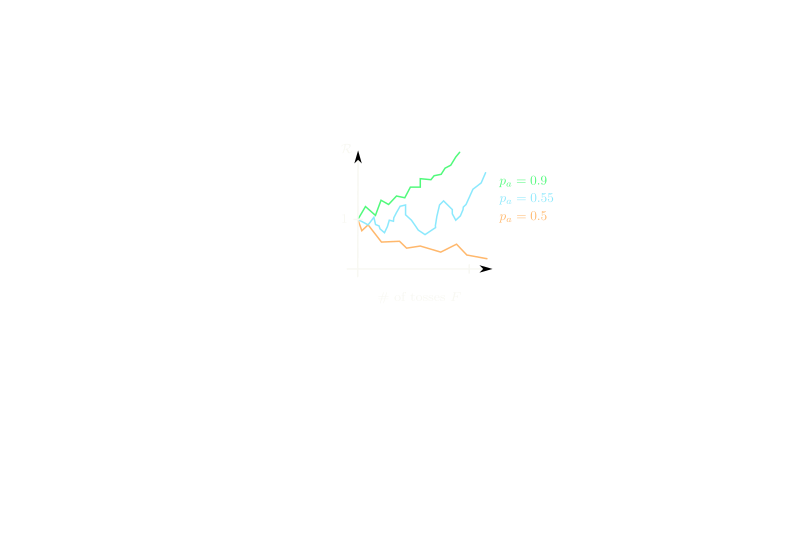
\includegraphics[width=0.5\textwidth]{images/bentcoin.png}
    \caption{Ratio of the two probabilities as a function of the number of tosses}
    \label{fig:bentcoin}
\end{figure}
where the the bent coin $p_a = 0.9$ probability goes to infinity as well as the slightly biased coin
(but at a slower pace) and the fair coin goes to zero. We know this from the probability
\begin{align*}
    P(s|F,H_o) = \int_0^1 P(s|p_a, F, H_1) P(p_a|F, H_1) dp_a
\end{align*} 
\emph{NOTE: There exists a $p_a$ that fits data better than $H_o$, but this evidence term includes
averaging over $p_a$}

Bayes theorem in the context of model comparison
\begin{align*}
    \textrm{bayes} = \frac{\textrm{likelihood} \cdot \textrm{prior}}{\textrm{evidence}}
\end{align*}

\emph{TAKEHOME: Bayesian model comparison naturally includes Occam's Razor!}

\paragraph{2.4} P-values? Why not just use p-values? e.g.
\begin{align*}
    F &= 250 \qquad F_a = 141, F_b = 109 \\
\end{align*}
Do these data suggest that the coin is biased? 

\paragraph{P-value:} Probability to get data as extreme or move, assuming the null hypothesis is
true. 
\begin{itemize}
    \item Null hypothesis: Coin is fair ($H_o$)
    \item Our hypothesis: Coin is biased ($H_1$)
    \item mean $= F/2$
    \item $\sigma = \sqrt{F}/2$
    \item Our observation: $\frac{F_a - F/2}{\sqrt{F}/2} = 2.02 \sigma$
    \item p-value $= 0.0497 < 0.05$!!!!
\end{itemize}
Google ``a small p-value ($<0.05$) indicates strong evidence against the null hypothesis so you
reject it''
% insert fig
\begin{figure}[ht]
    \centering
    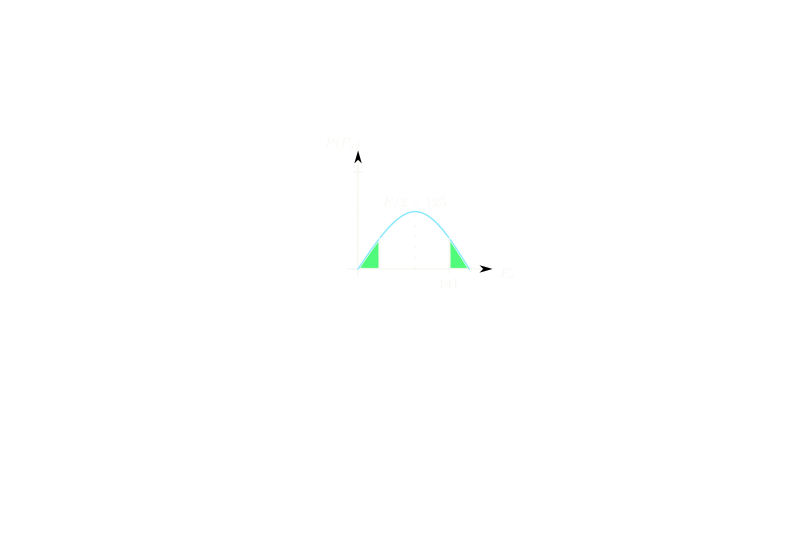
\includegraphics[width=0.5\textwidth]{pvalue.png}
    \caption{Finding p-value based on the Gaussian distribution}
    \label{fig:pvalue}
\end{figure}

From sterling approximation
\begin{align*}
    ln(k!) \approx k ln(k) - k + \dots
\end{align*}
With uniform prior on $p_a$
\begin{align*}
    \mathcal{R} = \frac{2^250 141! 109!}{251!} = 0.61
\end{align*}
if anything, there is weak evidence \emph{against} coin being biased.

\paragraph{Non-uniform priors?} For a reasonable family of priors, across the entire set of priors,
strongest evidence for bias is $2.5:1$ (From Mackay) This differs from the p-value which is $20:1$.

\section{Chapter 3: Maximum Likelihood \emph{Approximation}} (Ch 22 Mackay)

\paragraph{GOAL:} Connect to the stat you may have seen before. Going back to Example 4 (Urns and
more urns)

\begin{itemize}
    \item Unkown $u*$ selected at random
    \item 10 draws (with replacement): 3 black
    \item $P$(next draw $=$ black) $= ?$
    \item Most likeley $u: 3 \to$ predicts 0.3
    \item Correct answer: predicts 0.33
\end{itemize}
but the two numbers are kinda similar\dots 

\emph{NOTE: Bayesian model comparison, not model selection, but complete enumeration of
hypothesese (integration over hyp space) is computationally expensive (especially in high
dimensions)}

e.g. Comparing 2 models:
\begin{itemize}
    \item 1 Gaussian: 2 parameters $\mu, \sigma$
    \item 2 Gaussian ($a_1 G_1 + a_2 G_2$): 5 parameters $\mu_1, \sigma_1, \mu_2, \sigma_2, a_1/a_2$
\end{itemize}
This problem of an increasing number of parameters motivates \emph{Max likelihood (ML) 
approximation}: instead of enumeration, focus on \emph{1} hypothesis that maximized the likelihood
function.

\paragraph{Max Likelihood Estimation (MLE)} 
\begin{align*}
    P(\theta | D) = \frac{P(D | \theta) P(\theta)}{P(D)}
\end{align*}
instead of [assuming prior $\to$ compute posterior $\to$ integrate over hyp space] we just [compute 
the likelihoood unction $\to$ maximize it] (MLE).

\paragraph{3.1} A single Gaussian
\begin{itemize}
    \item Data: $\qt{x_n} \quad n = 1, \dots, N$
    \item model: these observations were sampled from a gaussian with probability
\begin{align*}
    P(x) = \frac{1}{\sqrt{2\pi \sigma^2}} e^{-\frac{(x - \mu)^2}{2\sigma^2}}
\end{align*}
    where we have 2 parameters $\mu, \sigma$ to determine.
\end{itemize}

\paragraph{Log likelihood} (multiplying likelihoods is hard, adding log likelihoods is easier)
\begin{align*}
    \ln P(\{x_n\} | \mu, \sigma) &= 
        \sum_{n=1}^N \qt(-\ln{\sqrt{2\pi \sigma^2}} - \frac{(x_n - \mu)^2}{2\sigma^2}) \\
    &= - N \ln{\sqrt{2\pi \sigma^2}} - \frac{N}{2\sigma^2} \sum_{n=1}^N (x_n - \mu)^2
\end{align*}

\paragraph{Sufficient statistics:} Denote
\begin{align*}
    \hat x &\equiv \sum_n \frac{x_n}{N} \qq{empirical mean} \\
    S &= \sum_n (x_n - \hat x)^2 \qq{sum of square deviations}
\end{align*}
These two numbers refer to the sufficient statistics. From these we get the log likelihood
\begin{align*}
    \ln P &= -N \ln{\sqrt{2\pi \sigma^2}} - \frac{N(\mu - \hat x)^2 + S}{2\sigma^2}
\end{align*}
Thus the max likelihood estimate of $\mu, \sigma$ are
\begin{align*}
    \mu_{ML} &= \hat x \\
    \sigma_{ML} &= \sqrt{\frac{S}{N}} = \sqrt{\frac{\sum_n (x_n - \hat x)^2}{N}} 
\end{align*}
If $\sigma$ is known, then $P(\mu)$ is a Gaussian we know that $\sigma/\sqrt{N}$ is the width of the
likelihood (error bars)

\newpage
\section*{Lecture 2/6/24}
\barh \vspace{10px}

\paragraph{Last time:} We discussed familiar stats.
\begin{itemize}
    \item Bayes Calculus in terms of $P(\theta)$ (params). Predictions of $x$
    \begin{align*}
        P(x) = P(x| \theta) P(\theta) d\theta \qqtext{is computationally hard}
    \end{align*}
    \item MLE: instead of full enumeration, focus on 1 hypothesis and its max likelihood
\end{itemize}
\paragraph*{3.1} Fitting a single Gaussian
\begin{align*}
    \theta = \qt{\sigma, \mu} \quad P(D|\theta) = \prod_n^N \frac{1}{\sqrt{2\pi \sigma^2}}
    \exp(-\frac{(x_n - \mu)^2}{2\sigma^2})
\end{align*}
we get the sufficient stats
\begin{align*}
    \mu_{ML} &= \hat x = \frac{\sum_i x_i}{N} \\
    \sigma_{ML} &= \sqrt{\frac{\sum_i (x_i - \hat x)^2}{N}}
\end{align*}
Beyond the MLE: we can get the error bars on $\mu$ AKA ``Standard error of the mean'': $\sigma/\sqrt{N}$


\subsubsection*{HW 2 HINTS}
\begin{itemize}
    \item MAX LIKELIHOOD WORKS (WELL) FOR PREDICTIONS/ ESTIMATES WHEN MOST OF THE PROB WEIGH IS NEAR
    THE ML ESTIMATE

    THIS IS NOT ALWAYS THE CASE! (most of the prob weight can be located not near the ML, Most
    of the prob weight is around the center)

    e.g. For two gaussian with 2 clusters, fitting the model with 1 gaussian may have a super narrow
    but the MLE will tend to that narrow peak even though the data is not near that peak.

    \item MOST LIKELY $\neq$ TYPICAL / REPRESENTATIVE (Mackay 22)
\end{itemize}

\paragraph{3.2} Least square fitting: e.g. linear fit
\begin{itemize}
    \item Dat: $\qt{y_n}$ for each $\qt{x_n}$
    \item Model: $y_n = a x_n + b +$ Gaussian noise of width $\sigma$
    \item Given $x_n, \sigma$, the params are $a, b$
\end{itemize}

\paragraph*{Model (more formally):}
\begin{align*}
    P(y_n | x_n, a, b, \sigma) = \prod_{n=1}^N \frac{1}{\sqrt{2\pi \sigma^2}}
    \exp(-\frac{(y_n - (a x_n + b))^2}{2\sigma^2})
\end{align*} 
How do I infer $a, b$ using the MLE: Log likelihood!
\begin{align*}
    \ln P = C - \sum_{n=1}^N \frac{(y_n - (a x_n + b))^2}{2\sigma^2}
\end{align*}
where $C$ is a constant, and we must maximize over $a, b$. Maximing $\ln P$ over $a, b$ is
equivalent to minimizing sum of squares of residuals (deviation of $y_n$ from the $a,b$). 

\begin{itemize}
    \item[!] (a) Not magic or ad hoc
    \item[!] (b) This is For Gaussian errors \emph{only} (of same magnitude).
    LSQ $\leftrightarrow$ Gaussian
\end{itemize}
\paragraph*{Takehome:} MLE is widely use \& often very sensible, but MLE $\neq$ not a silver bullet
especially in high dimensions! (e.g. HW2) 

\paragraph{Real world Example!} How sensitive are our eyes? 
\begin{itemize}
    \item Participants look at dim flashes in a dark room overa time $t$ with a height of the flash
    $A$ (brightness)
    \item How low can $A$ be for the flash to be detected?
    \item Experiemnt $E_1$: Flashes arrive randomly at some average rate. e.g. a flash but no response
    is a false negative while a false positive is a response but no flash (1 per 10 sec on average).
    \item Experiment $E_2$: First a bright pulse $A_o$ (or beep of possible oncoming flash) that is easy to see, then $1$ sec later, the 
    there is either a flash of heigh $A$ or no flash at all with prob $p$. 
\end{itemize}
In both cases, both make $A$ dimmer and measure for accuracy. We would expect that $E_2$ would allow
us to detect dimmer flashes since we can expect. 

\paragraph*{Ground truth} For $E_2$ when we know when to expect we let $f = 0$ as no flash
and $f = 1$ a flash. For the perfect detector and noisy detector we have Figure \ref{fig:flash}. 
There also exista abackground noise $b$ that is always present. 

\begin{figure}[ht]
    \centering
    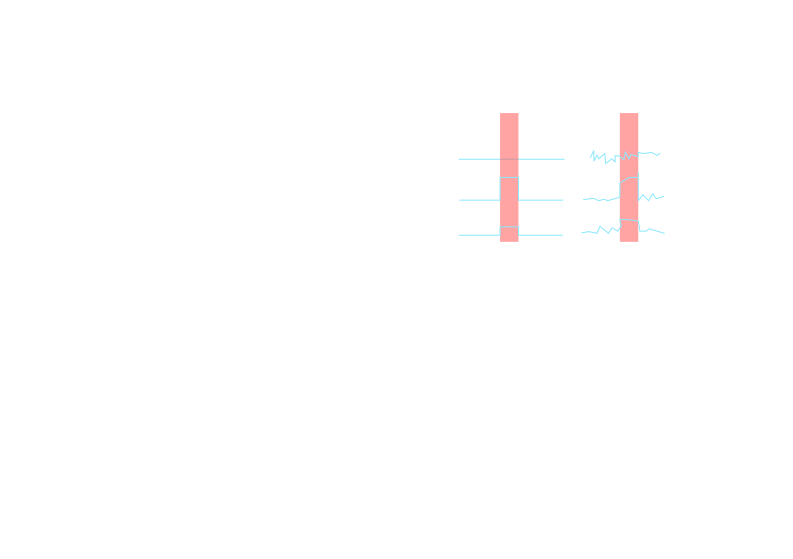
\includegraphics[width=0.5\textwidth]{images/sense.png}
    \caption{From top to bottom we have a no light $f=0$, and two cases of $f = 1$ for a bright
    light and dim light. The Pefect detector (left) sees and appropriates with the correct response
    while the noisy (Gaussian) detector may have a incorrect response (especially for the dimmer
    signal).}
    \label{fig:flash}
\end{figure}

\paragraph*{Data} For a noise time trace $I(t)$ over 5 seconds, we have a probability of a flash
$P(f) \approx  0.5$. 
\begin{align*}
    P(D | A, f, \eta, E_2) 
\end{align*}
with parameters $A; f, \eta$ and the simplest version: $A, \eta$ given an inference of $f$

\paragraph*{$E_2$} The hypothesis space we have either `Flash' or `No Flash'. The expected model is
a flash or no flash with Gaussian noise. We know the $A$
and $\eta$. The parameters to infer are $f = 0, 1$ and the inference questions is $f=?$

\paragraph*{$E_1$} The hypothesis: $H_1$ flash at $t$, $H_o$ no flash. The model has known: $A, \eta, b$.
Parameters: $f=0, 1$ and $t$. Inference question: $H_1$ or $H_o$? Figure \ref{fig:flash2} shows the 
expectation of the model. 

\begin{figure}[ht]
    \centering
    \includegraphics[width=0.5\textwidth]{visionmodel.png}
    \caption{The expectation of the models given experiment $E_1$ and $E_2$. The top is for 
    an expected model of a flash and no flash for bottom. NOTE that there also
    is Gaussian noise $\eta$ added to both scenerios.}
    \label{fig:flash2}
\end{figure}

\paragraph*{Approach} we have $P(D|\text{param}) \to$ Bayes' Theorem
\begin{itemize}
    \item $E_2$: Bayes' Theorem $\to P(f|D, \eta, A, b)$. If $f=1$ we are more likely to say we
    \emph{saw it} with an error probability: (average of the probability of making a mistake over
    all data including False Positives and False Negatives)
    \begin{align*}
        \langle P(\textrm{wrong f}|D, \eta, A, b) \rangle \qqtext{data}
    \end{align*}
    the error rate is a complicated integral (an average is a sum/trace/integral!): 
    \begin{align*}
        \textrm{Error rate}(A, \eta, b) = \int \dd{\text{data}} P(f=1|D) P(D|f=0,A,\eta)
    \end{align*}
\end{itemize}
\begin{figure}[ht]
    \centering
    \includegraphics[width=0.5\textwidth]{vmodel1.png}
    \caption{The error rate as a function of the brightness of the flash.}
    \label{fig:flash3}
\end{figure}

\paragraph*{Simpler approach?} We define $I^*$ as a mean intensity over a window of interest. 
For $E_2$ we can easily find the window of interst, but for $E_1$ we could discriminate the window
by finding the brightest flash and comparing it some threshold. Here lies two questions: how does a
computer that computes whether or not there is a flash versus a human that is looking for a flash
after 5 seconds.

\paragraph*{} If $\eta$ is known, $P(D|f,A,b)$ depends only on $I^*$ (sufficient statistics).

\paragraph*{Version 2:} Data: $I^*$ is just \emph{one} number. The probability given no flash or 
flash. Redefining noise $\eta$ as expected noise of measurement over window length. As shown in
Figure . 
\begin{figure}
    \centering
    \includegraphics[width=0.5\textwidth]{vision_v2.png}
    \caption{There is a shift in the no flash model in $E_1$}
    \label{fig:flash4}
\end{figure}

In $E_2$ we have a Gaussian distribution of the flash and no flash models, but in the $E_1$
the flash model is the same as we take the same window length of interest, but for the no flash model
the model moves to the right as we have a likelihood of measuring a window length with MORE noise. 
The error probability for $E_2$ is: Looking at the midpoint of the two models, we can find the error
as a sum of tail distribution (finding the weight of the outliers).
\begin{align*}
    \text{error} = \int_{A/2}^\infty \frac{1}{\sqrt{2\pi\eta^2} \exp(-\frac{x^2}{2\eta^2})} 
\end{align*}
the error is shown in Figure .
\begin{figure}[ht]
    \centering
    \includegraphics[width=0.5\textwidth]{v_error.png}
    \caption{The error rate as a function of amplitude $A$.}
    \label{fig:flash5}
\end{figure}
If human interaction is close to Bayesian $\to$ specific \emph{quant}
prediction for perfomance, effect of having the cue, rate of $P$.

\paragraph*{Takehomes}
\begin{itemize}
    \item What is data? (non-trivial question)
    \item What is hyp? (not unique)
    \item Most straightforward method can be impossible
    \item Under the hood: Still Bayesian calculus.
\end{itemize}

\newpage
\section*{Lecture 2/8/24}
\barh \vspace{10px}

\paragraph*{Is Science Solved?}
The steps of science:
\begin{enumerate}
    \item Gather Data + Build Model
    \item Fit each model to data
    \item Assign preferences to different models
    \item Either Method 1: Choose which data to gather next, gather more data, and back to step (2),or
    Method 2: Decide whether to create new model, create new model, and back to step (2)
\end{enumerate}

\paragraph*{The not 'just math' part:} Data $\to$ clever choice of features $\to$ model the
features/ model the noise.

\paragraph*{Takehomes:}
\begin{itemize}
    \item Choices in dataprocessing, Feature definitions, choice of data acquisition
    \item Depends on scieniic question: you need to know you subjective. Depends on the measurement:
    you need to know you experiment
\end{itemize}
Fly embyro patterning $=$ perfec example; astonishingly precise, thus the precision of data anaylsis
is the limiting factor

\paragraph*{Role:} Carries `positional information'

If I konw Hb (hunchback protein concentration), I know somthing about where I am; Hb and $x$ are not
independent. Nature (funnel shaped) vs. Cell (narrow tube shaped) article arguments.

\newpage
\section*{Lecture 2/15/24}
\barh \vspace{10px}
\paragraph*{Presentation: Entropy \& Mutual Info}
\paragraph*{takehome:} Information content in a random variable $X \rightleftharpoons$ Entropy
$H(X)$
\paragraph*{!} Not arbitrayry, but natural \& unique: Info content $H(X)$ has a \emph{discrete 
distribution}
\begin{itemize}
    \item[i] $H(\qt{p_i}) \geq 0$
    \item[ii] $H(\qt{p_i}) = 0$ iff $p_i = 1$ and others are 0
    \item[iii] If $X,Y$ are independent $Z=(X,Y)$ and $H(Z) = H(X) + H(Y)$
    \item[iv] $p_i = \qt{1/N, 1/N, \dots, 1/N}$, $H(X)$ should be monotonic in $N$
\end{itemize}
\paragraph*{Strengths of MI:} Not arbitrary: $X,Y$ are not independent, so $P(X) \neq P(X|Y)$
\begin{itemize}
    \item[i] $I(X;Y) = I(Y;X)$
    \item[ii] $I(X;Y) \leq H(X)$
    \item[iii] $I(X;Y) = 0$ iff $X,Y$ are independent
    \item[iv] If $X,Y$ are related deterministically, then $I(X;Y) = H(X) = H(Y)$
\end{itemize}
If we know that they are not indepenent $H(X,Y) = H(X|Y) + I(X,Y) + H(Y|X)$ and
$H(X,Y) \neq H(X) + H(Y)$ (there is overlap for dependent variables)
\paragraph*{MOST IMPORTANT THING:} Data processing inequality: ``Data processing can only destroy
information''. $X$ only knows about $Y$ and $Z$ only knows about $X$,
\begin{align*}
    X \to Y \to Z; \quad P(X,Y,Z) = P_x(X) P_y(Y|X) P_z(Z|Y)
\end{align*}
thus
\begin{align*}
    I(X;Y) \geq I(X;Z)
\end{align*}
\paragraph*{Weaknesses:}
\begin{itemize}
    \item[!] Estimating from data can require a lot of data.
    \item[!] Information $\neq$ Useful Information. i.e. pure noise can have a \emph{lot} of
    information
\end{itemize}

\newpage 
\section*{Lecture 2/20/24}
\barh \vspace{10px}

\paragraph*{Personal Thoughts:} When we make a decision we have to consider what happens to the
data explicitly. Normalizing does not make the data directly comparable to other data. Its easy to
identify noise, so we should think twice when we compare it to other things

\begin{itemize}
    \item Houchmandzadeh et al.: 
    Limitations of data $\to$ Data analysis (had a subtle flaw) $\to$ one Conclusion
    \item Gregor et al.
    Better data (very careful exp) $\to$ extrene careful data analysis $\to$ opposite conclusion.
\end{itemize}
\paragraph*{Takehomes:} 
\begin{itemize}
    \item Smart people make mistakes
    \item If it's too good to be true, it might be???
    \item Data is never what you think it is
    \item Details matter
\end{itemize}

\newpage
\section*{Lecture 2/22/24}
\barh \vspace{10px}

\paragraph*{Methods:} How did we collect the data?
\begin{table}[ht]
    \centering
    \begin{tabular}{c c c}
        & Nature & Cell \\
        \hline 
        Microscope & Scanning Confocal & Scanning Two Photon \\
        Embryo & Fixed (dead) & Live \\
        Labeling & Immunostaining & ``Bcd-GFP'' fusion protein \\
    \end{tabular}
\end{table}
\paragraph*{}
How to attach fluorophores 101:
\paragraph*{Immunostaining:} Washing off too much could wash off the pertinant proteins. It is
washed multiple times to get rid of the background fluorescence. When we wash with the neutral
buffer saline. First the Primary antibody (Ab) is washed off, then the second Ab, anti-rabbit, is
washed off. TLDR; Fix, label, wash
\begin{itemize}
    \item Strengths: Multiple washes leads to more(amplify) signal
    ; Not genetic engineering (easier); more colors!; dead sometimes an advantage for
    storage

    \item Weaknesses: Multiple washes leads to more background fluorescence; The wash may dilute?;
    amplifies unevenly; both random and systematic (place in cell); dead; fixation leads to
    deformation, shrinking, etc.
\end{itemize}
\paragraph*{Protein fusion} Genetically modify the fly to have GFP (Green Fluorescent Protein) fused
to the protein of interest. TLDR; Engineer, add to protein of interest + GFP.
\begin{itemize}
    \item Strengths: we're not adding wash; it's alive!; direct readout
    \item Weaknesses: GFP not bright? Limited Fluorophores (The fly has to make the bright stuff), 
    ,so less bright less photostable; does the fusion protein still work the same?
\end{itemize}
Fluorescescing too much can lead to bleaching (death) of the protein. What kind of fluorophore is
being used?

\paragraph*{Errors \& Noise:} Fixed: Variable age at collection, mechanical deform, labeling efficiency
(targets or not targets are labeled). Live: GFP can alter function, Impact by details of cell
environment (maturation time of fluoresce). 

\paragraph*{Microscope \& Imaging:} Laser shoots stuff to scanning (moving mirrors) and a
fluorescence detector collects data. 

\paragraph*{Confocal:} Only stuff in the focal plane is collected (closer and further stuff is out
of focus). Everything in the laser is fluorescing and fluorophores have a limited lifetime(can 
bleach quicker).

\paragraph*{Two Photon:} Infrared laser only excites the fluorophores in the place we want. In the
image, the outside part has an exact concentration, so we can compare this to the inside part.

\paragraph*{Takehomes:} Expression of Protein vs Position in Embryo (the canonical example): Is
15 embryos enought? Is 1000 embryos enough? Looking at this picture: here is a plot, but is this
the position in the embryo? no, it's the position in the image. Is it a picture of the image? no,
its a picutre of 1D projection of the image. Is this expression? no, its tagged ptoteins... no its
fluorescences... no its pixel values! More steps, more noise, more errors, there is complexity! 
The subject expert has the role to give us the answers to these questions. I don't know what the
microscope is doing is bad!
\end{document}